\documentclass[nooutcomes]{ximera}
\input{../preamble.tex}


\author{Elizabeth Miller, Kenneth Berglund}
%\license{Creative Commons 4.0 International License}



\title{Famous Functions, Updated}

\begin{document}

\begin{abstract}
\end{abstract}
\maketitle

%\typeout{************************************************}
%\typeout{Famous Functions and Relations}
%\typeout{************************************************}

%\section{Famous Functions and Relations} 
Now that we know about the domain and range, we can update our list of famous functions. 

\newpage

In Section 1-2, you saw a variety of famous functions. Now that we have learned more about properties of functions, we can update our knowledge of those famous functions. We will go through the list of famous functions from before and point out where each function might have properties we've discussed.

\newpage

%\typeout{************************************************}
%\typeout{Linear Functions}
%\typeout{************************************************}

\section{Linear Functions}
Recall that the graph of a linear function is a line. 

\begin{example}
A prototypical example of a linear function is 

\begin{center}
  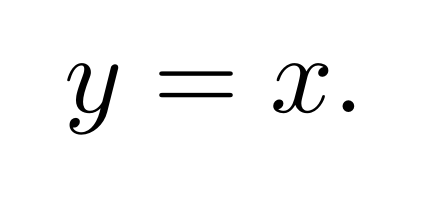
\begin{tikzpicture}[scale=4,every node/.style={transform shape}]
    \node at (0,0) {$y=x.$};
  \end{tikzpicture}
\end{center}

\begin{center}
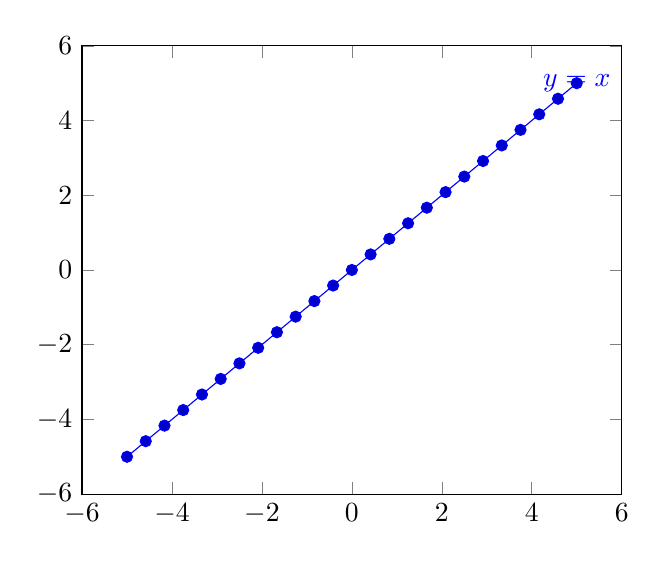
\begin{tikzpicture}
    \begin{axis}
        \addplot{x} node{$y=x$};
    \end{axis}
\end{tikzpicture}
\end{center}


\[
\begin{array}{  c  }
 %\hline
\text{\normalfont Important Values of $y=x$} \\
 \begin{array}{|c|c|}
 \hline
 x & y\\
 \hline
 -2&-2\\
 -1&-1\\
 0&0\\
 1&1\\
 2&2\\
 \hline
\end{array}
\end{array}
\]

\end{example}

In general, linear functions can be written as $y=mx+b$ where $m$ and $b$ can be any numbers. We learned that $m$ represents the slope, and $b$ is the $y$-coordinate of the $y$-intercept. You can play with changing the values of $m$ and $b$ on the graph using Desmos and see how that changes the line.  

\begin{center}  
\desmos{japnhapzvn}{800}{600}  
\end{center}

Note that a linear function $f$ defined by $f(x) = mx + b$ with $b = 0$ is odd. If $m = 0$, then $f$ is periodic, since it is constant. Furthermore, constant functions are always even.

Additionally, if $m \ne 0$, then a linear function is one-to-one, and therefore invertible. We summarize this information in the table below.


Note that any real number can be plugged into $f(x) = mx + b$, so the domain of linear functions is $(-\infty, \infty)$. Unless $m = 0$, we can find a $y$ such that $y = mx + b$, so the range of linear functions with $m \ne 0$ is $(-\infty, \infty)$. If $m = 0$, then the only output of the linear function is $b$, so its range is $\{b\}$. 

\[
\begin{array}{  c  }
 %\hline
\text{\normalfont Properties of Linear Functions} \\
 \begin{array}{|c|c|}
 \hline
\text{Periodic?} & \text{If } m = 0 \\ \hline
\text{Odd?} & \text{If } b = 0 \\ \hline
\text{Even?} & \text{If } m = 0 \\ \hline
\text{One-to-one/invertible?} & \text{Yes}\\ \hline
\text{Domain} & (-\infty,\infty)\\ \hline
\text{Range} & (-\infty,\infty)\\ \hline
\end{array}
\end{array}
\]

\newpage

%\typeout{************************************************}
%\typeout{Quadratic Functions}
%\typeout{************************************************}

\section{Quadratic Functions}

Recall that the graph of a quadratic function is a parabola.

\begin{example}
A prototypical example of a quadratic function is 

\begin{center}
  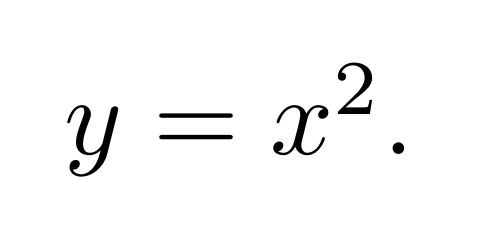
\begin{tikzpicture}[scale=4,every node/.style={transform shape}]
    \node at (0,0) {$y=x^2.$};
  \end{tikzpicture}
\end{center}

\begin{center}
\begin{tikzpicture}
    \begin{axis}
        \addplot[smooth]{x^2} node{$y=x^2$};
    \end{axis}
\end{tikzpicture}
\end{center}

\[
\begin{array}{c  }
 %\hline
\text{\normalfont Important Values of $y=x^2$} \\
 \begin{array}{|c|c|}
 \hline
 x & y\\
 \hline
 -2&4\\
 -1&1\\
 0&0\\
 1&1\\
 2&4\\
 \hline
\end{array}
\end{array}
\]
\end{example}

In general, quadratic functions can be written as $y=ax^2+bx+c$ where $a$, $b$, and $c$ can be any numbers.  You can play with changing the values of $a$, $b$, and $c$ on the graph using Desmos and see how that changes the parabola.  

\begin{center}  
\desmos{nmlghfrws9}{800}{600}  
\end{center}

Note that for a quadratic function $f$ defined by $f(x) = ax^2 + bx + c$, if $b = 0$, then $f$ is even. In general, quadratic functions are not one-to-one, odd, or periodic, except in cases where $a = 0$, in which we're actually dealing with a linear function. 

Note that any real number can be plugged into $f(x) = ax^2 + bx + c$, so the domain of quadratic functions is $(-\infty, \infty)$. In Chapter 4, we saw that all quadratic functions have a vertex form $f(x) = a(x - h)^2 + k$, where the vertex is at $(h, k)$. If $a > 0$, all points above the vertex, that is $[k, \infty)$ are in the range of the quadratic, and if $a < 0$, all points below the vertex, that is $(\infty, k]$ are in the range of the quadratic.

We summarize this information in the table below.

\[
\begin{array}{  c  }
 %\hline
\text{\normalfont Properties of Quadratic Functions } y=ax^2 + bx + c, a \ne 0 \\
 \begin{array}{|c|c|}
 \hline
\text{Periodic?} & \text{No} \\ \hline
\text{Odd?} & \text{No} \\ \hline
\text{Even?} & \text{If } b = 0 \\ \hline
\text{One-to-one/invertible?} & \text{No}\\ \hline
\text{Domain} & (-\infty,\infty)\\ \hline
\text{Range} & \text{If }a > 0\text{, } [k,\infty) \text{, if }a < 0\text{, } (-\infty, k]\\ \hline
\end{array}
\end{array}
\]



\newpage

%\typeout{************************************************}
%\typeout{Absolute Value Function}
%\typeout{************************************************}

\section{Absolute Value Function}
Another important type of function is the absolute value function.  This is the function that takes all $y$-values and makes them positive.  The absolute value function is written as 

\begin{center}
  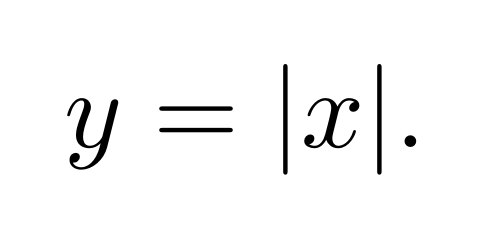
\begin{tikzpicture}[scale=4,every node/.style={transform shape}]
    \node at (0,0) {$y=|x|.$};
  \end{tikzpicture}
\end{center}

\begin{center}
\begin{tikzpicture}
    \begin{axis}
        \addplot[samples=200,domain=0:8]{x};
        \addplot[samples=200,domain=-8:0]{-x};
    \end{axis}
\end{tikzpicture}
\end{center}

\[
\begin{array}{c }
\text{\normalfont Important Values of $y=|x|$} \\
\begin{array}{|c|c|}
 \hline
 x & y\\
 \hline
 -2&2\\ 
-1&1\\ 
0&0\\
 1&1\\
 2&2\\
 \hline
\end{array}
\end{array}
\]

Notice that the absolute value function is even. Is it one-to-one? The fact that it's even tells us that it is not, since $|-x| = |x|$ for all $x$. We summarize this information in the table below.


Note that any real number has an absolute value, so the domain of the absolute value function is $(-\infty, \infty)$. Furthermore, by looking at the graph, we can see that all non-negative numbers are in the range of the absolute value function.

\[
\begin{array}{c }
\text{\normalfont Properties of the Absolute Value Function } y=|x| \\
\begin{array}{|c|c|}
 \hline
\text{Periodic?} & \text{No} \\ \hline
\text{Odd?} & \text{No} \\ \hline
\text{Even?} & \text{Yes } \\ \hline
\text{One-to-one/invertible?} & \text{No}\\ \hline
\text{Domain} & (-\infty,\infty)\\ \hline
\text{Range} & [0,\infty)\\ \hline
\end{array}
\end{array}
\]


\newpage

%\typeout{************************************************}
%\typeout{Square Root Function}
%\typeout{************************************************}

\section{Square Root Function}
Another famous function is the square root function,

\begin{center}
  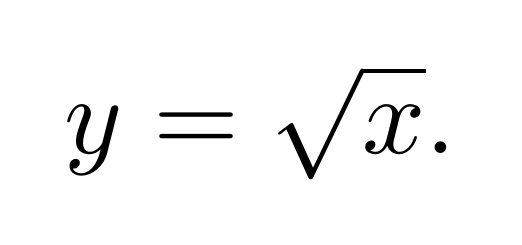
\begin{tikzpicture}[scale=4,every node/.style={transform shape}]
    \node at (0,0) {$y=\sqrt{x}.$};
  \end{tikzpicture}
\end{center}

\begin{center}
\begin{tikzpicture}
    \begin{axis}
        \addplot[samples=200,domain=0:30]{sqrt(x)};
    \end{axis}
\end{tikzpicture}
\end{center}


\[
\begin{array}{c }
 \text{\normalfont Important Values of $y=\sqrt{x}$} \\
\begin{array}{|c|c|}
 \hline
 x & y\\
 \hline
 0&0\\
 1&1\\
 4&2\\
 9&3\\
 25&5\\
 \hline
\end{array}
\end{array}
\]

The square root function is one-to-one. Negative inputs are not valid for the square root function, so it is neither even, odd, nor periodic. We summarize this information in the table below.

Note that only non-negative numbers have square roots, so the domain of the square root function is $[0, \infty)$. Furthermore, by looking at the graph, we can see that all non-negative numbers are in the range of the square root function. Algebraically, we can say that for any non-negative $y$, $\sqrt(y^2) = y$, so $y$ is in the range of the square root function.

\[
\begin{array}{c }
 \text{\normalfont Properties of the Square Root Function } y=\sqrt{x} \\
\begin{array}{|c|c|}
 \hline
\text{Periodic?} & \text{No} \\ \hline
\text{Odd?} & \text{No} \\ \hline
\text{Even?} & \text{No} \\ \hline
\text{One-to-one/invertible?} & \text{Yes}\\ \hline
\text{Domain} & [0,\infty)\\ \hline
\text{Range} & [0,\infty)\\ \hline
\end{array}
\end{array}
\]

\newpage

%\typeout{************************************************}
%\typeout{Exponential Functions}
%\typeout{************************************************}

\section{Exponential Functions}
Another famous function is the exponential growth function,

\begin{center}
  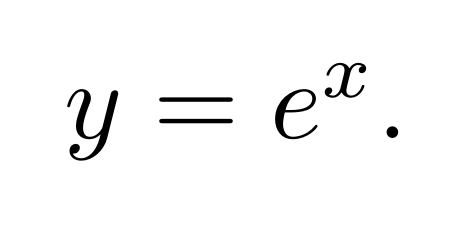
\begin{tikzpicture}[scale=4,every node/.style={transform shape}]
    \node at (0,0) {$y=e^{x}.$};
  \end{tikzpicture}
\end{center}


Here $e$ is the mathematical constant known as Euler's number.  $e \approx 2.71828 .$.

\begin{center}
\begin{tikzpicture}
    \begin{axis}
        \addplot[samples=200,domain=-10:4]{e^x};
    \end{axis}
\end{tikzpicture}
\end{center}

\[
\begin{array}{c}
 \text{\normalfont Important Values of } y=e^x \\
\begin{array}{|c|c|}
\hline
 x & y \\
 \hline 
 0&1\\[2ex]
 1&e\\[2ex]
 -1&e^{-1}=\frac{1}{e}\\[2ex]
\hline
\end{array}
\end{array}
 \]


In general, we can talk about exponential functions of the form $y=b^{x}$ where $b$ is a positive number not equal to $1$.  You can play with changing the values of $b$ on the graph using Desmos and see how that changes the graph.  Pay particular attention to the difference between $b>1$ and $0<b<1$.

\begin{center}  
%\desmos{dgcwh0chfv}{800}{600}  
\desmos{qsmvb7tiex}{800}{600}
\end{center}

Notice that exponential functions are one-to-one, and therefore invertible. However, they are neither even, odd, nor periodic. 

Note that the domain of the exponential functions is $(-\infty, \infty)$. Furthermore, by looking at the graph, we can see that all non-negative numbers are in the range of the exponential functions.

We summarize this information in the table below.

\[
\begin{array}{c}
 \text{\normalfont Properties of the Exponential Functions } y=b^x \\
\begin{array}{|c|c|}
\hline
\text{Periodic?} & \text{No} \\ \hline
\text{Odd?} & \text{No} \\ \hline
\text{Even?} & \text{No} \\ \hline
\text{One-to-one/invertible?} & \text{Yes} \\ \hline
\text{Domain} & (-\infty,\infty)\\ \hline
\text{Range} & (0,\infty)\\ \hline
\end{array}
\end{array}
 \]



\newpage

%\typeout{************************************************}
%\typeout{Logarithm Functions}
%\typeout{************************************************}

\section{Logarithm Functions}
Another group of famous functions are logarithms.

\begin{example}
The most famous logarithm function is
 $$ \mbox{\huge $y=\ln(x)=\log_{e}(x)$.}$$ 
Here $e$ is the mathematical constant known as Euler's number. $e \approx 2.71828$.

\begin{center}
\begin{tikzpicture}
    \begin{axis}
        \addplot[samples=200,domain=0.01:8]{ln(x)};
    \end{axis}
\end{tikzpicture}
\end{center}


\[
\begin{array}{ c  }
% \hline
  \text{Important Values of $y=\ln(x)$}\\
 \begin{array}{|c|c|}
 \hline
 x & y\\
 \hline
0&\text{undefined}\\[2ex]
\frac{1}{e}&-1\\[2ex]
1&0\\[2ex]
e&1\\[2ex]
 \hline
 \end{array}
\end{array}
 \]

\end{example}

In general, we can talk about logarithmic functions of the form $y=\log_b(x)$ where $b$ is a positive number not equal to $1$.  You can play with changing the values of $b$ on the graph using Desmos and see how that changes the graph.  Pay particular attention to the difference between $b>1$ and $0<b<1$.

\begin{center}  
\desmos{lxllnpdi6w}{800}{600}  
\end{center}

Notice that logarithms are neither even, odd, nor periodic. However, they are one-to-one, and therefore invertible. It turns out that the inverse of a logarithm is an exponential function, and vice versa! 

Note that since the logarithm is the inverse of the exponential, the domain of the logarithms is the range of the exponentials: $[0, \infty)$. Furthermore, the range of the logarithms is the range of the exponentials: $(-\infty, \infty)$. 

We summarize this information in the table below.

\[
\begin{array}{ c  }
% \hline
  \text{\normalfont Properties of the Logarithm Functions } y=\log_b(x)\\
 \begin{array}{|c|c|}
 \hline
\text{Periodic?} & \text{No} \\ \hline
\text{Odd?} & \text{No} \\ \hline
\text{Even?} & \text{No} \\ \hline
\text{One-to-one/invertible?} & \text{Yes} \\ \hline
\text{Domain} & (0,\infty)\\ \hline
\text{Range} & (-\infty,\infty)\\ \hline
 \end{array}
\end{array}
 \]


\newpage

%\typeout{************************************************}
%\typeout{Sine}
%\typeout{************************************************}

\section{Sine}
Another important function is the sine function, 

\begin{center}
  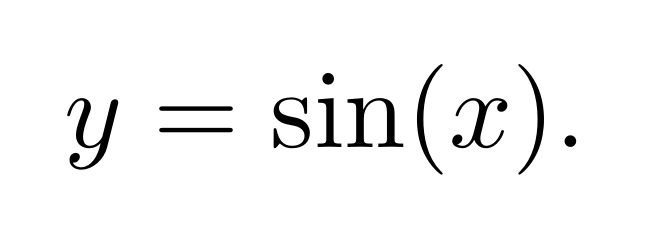
\begin{tikzpicture}[scale=4,every node/.style={transform shape}]
    \node at (0,0) {$y=\sin(x).$};
  \end{tikzpicture}
\end{center}



This function comes from trigonometry. In the table below we will use another mathematical constant, $\pi$ (``pi" pronounced pie). $\pi \approx 3.14159$.

\begin{center}
\begin{tikzpicture}
    \begin{axis}[ymin=-2, ymax=2,
           %xtick={-6.28318, -4.7123889, -3.14159, -1.5708, 1.5708, 3.14159, 4.7123889, 6.28318},
    xticklabels={
        $-\frac{3\pi}{2}$, $-\pi$, $\frac{\pi}{2}$, $0$,
        $\frac{\pi}{2}$, $\pi$, $\frac{3\pi}{2}$, $2\pi$
    }, ]
        \addplot[samples=200]{sin(pi/4*deg(x))};
    \end{axis}
\end{tikzpicture}
\end{center}

\[
\begin{array}{ c }
 \text{ Important Values of  $y=\sin(x)$}\\
\begin{array}{|c|c|}
 \hline
 x & y\\
 \hline
 -\pi&0\\[2ex]
 -\frac{\pi}{2}&-1\\[2ex]
 0&0\\[2ex]
 \frac{\pi}{2}&1\\[2ex]
 \pi&0\\[2ex]
\frac{3\pi}{2}&-1\\[2ex]
 2 \pi&0\\[2ex]
\hline
\end{array}
\end{array}
\]


As mentioned earlier, the sine function is odd and periodic with period $2\pi$. Since it is periodic, however, it cannot be one-to-one, since its values repeat. 

Note that the domain of the sine function is $(-\infty, \infty)$. Furthermore, by looking at the graph, we can see that its range is $[-1, 1]$.

We summarize this information in the table below.


\[
\begin{array}{ c }
 \text{\normalfont Properties of the Sine Function } y=\sin(x) \\
\begin{array}{|c|c|}
 \hline
\text{Periodic?} & \text{Yes, with period }2\pi \\ \hline
\text{Odd?} & \text{Yes} \\ \hline
\text{Even?} & \text{No} \\ \hline
\text{One-to-one/invertible?} & \text{No} \\ \hline
\text{Domain} & (-\infty,\infty)\\ \hline
\text{Range} & [-1,1]\\ \hline
\end{array}
\end{array}
\]

In general, we can consider $y=a\sin(bx)$.  You can play with changing the values of $a$ and $b$ on the graph using Desmos and see how that changes the graph.  

\begin{center}  
\desmos{vkxzcfv2aq}{800}{600}  
\end{center}



\newpage

%\typeout{************************************************}
%\typeout{Cosine}
%\typeout{************************************************}

\section{Cosine}
A function introduced in Section 3-2 is the cosine function, 

\begin{center}
  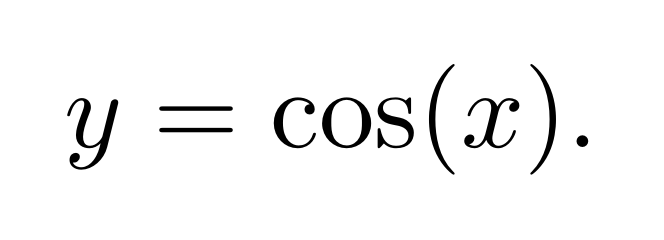
\begin{tikzpicture}[scale=4,every node/.style={transform shape}]
    \node at (0,0) {$y=\cos(x).$};
  \end{tikzpicture}
\end{center}


As with sine, the cosine function comes from trigonometry. In the table below we will again use $\pi$.

\begin{center}
\begin{tikzpicture}
    \begin{axis}[ymin=-2, ymax=2,
		   %xtick={-6.28318, -4.7123889, -3.14159, -1.5708, 1.5708, 3.14159, 4.7123889, 6.28318},
    xticklabels={
        $-\frac{3\pi}{2}$, $-\pi$, $\frac{\pi}{2}$, $0$,
        $\frac{\pi}{2}$, $\pi$, $\frac{3\pi}{2}$, $2\pi$
    }, ]
        \addplot[samples=200]{cos(pi/4*deg(x))};
    \end{axis}
\end{tikzpicture}
\end{center}

\[
\begin{array}{ c }
 \text{ Important Values of  $y=\cos(x)$}\\
\begin{array}{|c|c|}
 \hline
 x & y\\
 \hline
 -\pi&-1\\[2ex]
 -\frac{\pi}{2}&0\\[2ex]
 0&1\\[2ex]
 \frac{\pi}{2}&0\\[2ex]
 \pi&-1\\[2ex]
\frac{3\pi}{2}&0\\[2ex]
 2 \pi&1\\[2ex]
\hline
\end{array}
\end{array}
\]

As mentioned earlier, the cosine function is even and periodic with period $2\pi$. Since it is periodic, however, it cannot be one-to-one, since its values repeat. 


Note that the domain of the cosine function is $(-\infty, \infty)$. Furthermore, by looking at the graph, we can see that its range is $[-1, 1]$.

We summarize some information in the table below.

\[
\begin{array}{ c }
 \text{\normalfont Properties of the Cosine Function } y=\cos(x) \\
\begin{array}{|c|c|}
 \hline
\text{Periodic?} & \text{Yes, with period }2\pi \\ \hline
\text{Odd?} & \text{No} \\ \hline
\text{Even?} & \text{Yes} \\ \hline
\text{One-to-one/invertible?} & \text{No} \\ \hline
\text{Domain} & (-\infty,\infty)\\ \hline
\text{Range} & [-1,1]\\ \hline
\end{array}
\end{array}
\]

In general, we can consider $y=a\cos(bx)$.  You can play with changing the values of $a$ and $b$ on the graph using Desmos and see how that changes the graph.  

\begin{center}  
\desmos{kvmz1kt19n}{800}{600}  
\end{center}

%\typeout{************************************************}
%\typeout{Linear Functions}
%\typeout{************************************************}

%\section{Linear Functions}
%Recall that the graph of a linear function is a line. 
%
%\begin{example}
%A prototypical example of a linear function is $$ \mbox{\huge $y=x.$}$$ 
%
%\begin{image}
%\begin{tikzpicture}
%    \begin{axis}
%        \addplot{x} node{$y=x$};
%    \end{axis}
%\end{tikzpicture}
%\end{image}
%
%\begin{center}
%\(
%\begin{array}{ |c || c|  }
% \hline
% \multicolumn{2}{|c|}{\text{\normalfont Important Values of } y=x} \\
%\hline
% \hline
% x & y\\
% \hline
% -2&-2\\
% -1&-1\\
% 0&0\\
% 1&1\\
% 2&2\\
% \hline
%\end{array}
%\)
%\end{center}
%\end{example}
%
%In general, linear functions can be written as $y=mx+b$ where $m$ and $b$ can be any numbers. We learned that $m$ represents the slope, and $b$ is the $y$-coordinate of the $y$-intercept. You can play with changing the values of $m$ and $b$ on the graph using Desmos and see how that changes the line.  
%
%\begin{center}  
%\desmos{japnhapzvn}{800}{600}  
%\end{center}
%
%\begin{center}
%$
%\begin{array}{|l|l|}
% \hline
% \multicolumn{2}{|c|}{\text{\normalfont Properties of Linear Functions } y=mx + b} \\
%\hline
% \hline
%\text{Periodic?} & \text{If } m = 0 \\ \hline
%\text{Odd?} & \text{If } b = 0 \\ \hline
%\text{Even?} & \text{If } m = 0 \\ \hline
%\text{One-to-one/invertible?} & \text{Yes}\\ \hline
%\end{array}
%$
%\end{center}
%
%Note that any real number can be plugged into $f(x) = mx + b$, so the domain of linear functions is $(-\infty, \infty)$. Unless $m = 0$, we can find a $y$ such that $y = mx + b$, so the range of linear functions with $m \ne 0$ is $(-\infty, \infty)$. If $m = 0$, then the only output of the linear function is $b$, so its range is $\{b\}$. 
%
%
%\begin{center}
%$
%\begin{array}{|l|l|}
% \hline
% \multicolumn{2}{|c|}{\text{\normalfont Domain and Range of Linear Functions } y=mx + b} \\
%\hline
% \hline
%\text{Domain} & (-\infty, \infty) \\ \hline
%\text{Range} & \text{If } m \ne 0\text{, } (-\infty, \infty)\text{; if } m = 0 \text{, } \{b\}\\ \hline
%\end{array}
%$
%\end{center}
%
%
%\newpage
%
%%\typeout{************************************************}
%%\typeout{Quadratic Functions}
%%\typeout{************************************************}
%
%\section{Quadratic Functions}
%
%Recall that the graph of a quadratic function is a parabola.
%
%\begin{example}
%A prototypical example of a quadratic function is $$ \mbox{\huge $y=x^2.$}$$
%
%\begin{image}
%\begin{tikzpicture}
%    \begin{axis}
%        \addplot[smooth]{x^2} node{$y=x^2$};
%    \end{axis}
%\end{tikzpicture}
%\end{image}
%
%\begin{center}
%\(
%\begin{array}{ |c || c|  }
% \hline
% \multicolumn{2}{|c|}{\text{\normalfont Important Values of } y=x^2} \\
%\hline
% \hline
% x & y\\
% \hline
% -2&4\\
% -1&1\\
% 0&0\\
% 1&1\\
% 2&4\\
% \hline
%\end{array}
%\)
%\end{center}
%\end{example}
%
%In general, quadratic functions can be written as $y=ax^2+bx+c$ where $a$, $b$, and $c$ can be any numbers.  You can play with changing the values of $a$, $b$, and $c$ on the graph using Desmos and see how that changes the parabola.  
%
%\begin{center}  
%\desmos{nmlghfrws9}{800}{600}  
%\end{center}
%
%\begin{center}
%$
%\begin{array}{|l|l|}
% \hline
% \multicolumn{2}{|c|}{\text{\normalfont Properties of Quadratic Functions } y=ax^2 + bx + c, a \ne 0} \\
%\hline
% \hline
%\text{Periodic?} & \text{No} \\ \hline
%\text{Odd?} & \text{No} \\ \hline
%\text{Even?} & \text{If } b = 0 \\ \hline
%\text{One-to-one/invertible?} & \text{No}\\ \hline
%\end{array}
%$
%\end{center}
%
%Note that any real number can be plugged into $f(x) = ax^2 + bx + c$, so the domain of quadratic functions is $(-\infty, \infty)$. In Chapter 4, we saw that all quadratic functions have a vertex form $f(x) = d(x - h)^2 + k$, where the vertex is at $(h, k)$. If $d > 0$, all points above the vertex, that is $[k, \infty)$ are in the range of the quadratic, and if $d < 0$, all points below the vertex, that is $(\infty, k]$ are in the range of the quadratic.
%
%\begin{center}
%$
%\begin{array}{|l|l|}
% \hline
% \multicolumn{2}{|c|}{\text{\normalfont Domain and Range of Quadratic Functions } y=d(x - h)^2 + k} \\
%\hline
% \hline
%\text{Domain} & (-\infty, \infty) \\ \hline
%\text{Range} & \text{If } d > 0\text{, }[k, \infty)\text{; if }d < 0\text{, }(\infty, k]\\ \hline
%\end{array}
%$
%\end{center}
%
%\newpage
%
%%\typeout{************************************************}
%%\typeout{Absolute Value}
%%\typeout{************************************************}
%
%\section{Absolute Value}
%Another important type of function is the absolute value function.  This is the function that takes all $y$-values and makes them positive.  The absolute value function is written as 
%
%$$ \mbox{\huge $y=|x|.$}$$ 
%
%\begin{image}
%\begin{tikzpicture}
%    \begin{axis}
%        \addplot[smooth]{abs(x)} node{$y=|x|$};
%    \end{axis}
%\end{tikzpicture}
%\end{image}
%
%\begin{center}
%\(
%\begin{array}{ |c || c|  }
% \hline
% \multicolumn{2}{|c|}{\text{\normalfont Important Values of } y=|x|} \\
%\hline
% \hline
% x & y\\
% \hline
% -2&2\\ 
%-1&1\\ 
%0&0\\
% 1&1\\
% 2&2\\
% \hline
%\end{array}
%\)
%\end{center}
%
%\begin{center}
%$
%\begin{array}{|l|l|}
% \hline
% \multicolumn{2}{|c|}{\text{\normalfont Properties of the Absolute Value Function } y=|x|} \\
%\hline
% \hline
%\text{Periodic?} & \text{No} \\ \hline
%\text{Odd?} & \text{No} \\ \hline
%\text{Even?} & \text{Yes } \\ \hline
%\text{One-to-one/invertible?} & \text{No}\\ \hline
%\end{array}
%$
%\end{center}
%
%Note that any real number has an absolute value, so the domain of the absolute value function is $(-\infty, \infty)$. Furthermore, by looking at the graph, we can see that all non-negative numbers are in the range of the absolute value function.
%
%\begin{center}
%$
%\begin{array}{|l|l|}
% \hline
% \multicolumn{2}{|c|}{\text{\normalfont Domain and Range of the Absolute Value Function } y=|x|} \\
%\hline
% \hline
%\text{Domain} & (-\infty, \infty) \\ \hline
%\text{Range} & [0, \infty)\\ \hline
%\end{array}
%$
%\end{center}
%
%\newpage
%
%%\typeout{************************************************}
%%\typeout{Square Root}
%%\typeout{************************************************}
%
%\section{Square Root}
%Another famous function is the square root function, $$ \mbox{\huge $y=\sqrt{x}.$}$$ 
%
%\begin{image}
%\begin{tikzpicture}
%    \begin{axis}
%        \addplot[samples=200,domain=0:30]{sqrt(x)};
%    \end{axis}
%\end{tikzpicture}
%\end{image}
%
%
%\begin{center}
%\(
%\begin{array}{ |c || c|  }
% \hline
% \multicolumn{2}{|c|}{\text{\normalfont Important Values of } y=\sqrt{x}} \\
%\hline
% \hline
% x & y\\
% \hline
% 0&0\\
% 1&1\\
% 4&2\\
% 9&3\\
% 25&5\\
% \hline
%\end{array}
%\)
%\end{center}
%
%\begin{center}
%$
%\begin{array}{|l|l|}
% \hline
% \multicolumn{2}{|c|}{\text{\normalfont Properties of the Square Root Function } y=\sqrt{x}} \\
%\hline
% \hline
%\text{Periodic?} & \text{No} \\ \hline
%\text{Odd?} & \text{No} \\ \hline
%\text{Even?} & \text{No} \\ \hline
%\text{One-to-one/invertible?} & \text{Yes}\\ \hline
%\end{array}
%$
%\end{center}
%
%Note that only non-negative numbers have square roots, so the domain of the square root function is $[0, \infty)$. Furthermore, by looking at the graph, we can see that all non-negative numbers are in the range of the square root function. Algebraically, we can say that for any non-negative $y$, $\sqrt(y^2) = y$, so $y$ is in the range of the square root function. 
%
%\begin{center}
%$
%\begin{array}{|l|l|}
% \hline
% \multicolumn{2}{|c|}{\text{\normalfont Domain and Range of the Square Root Function } y=\sqrt{x}} \\
%\hline
% \hline
%\text{Domain} & [0, \infty) \\ \hline
%\text{Range} & [0, \infty) \\ \hline
%\end{array}
%$
%\end{center}
%
%%\typeout{************************************************}
%%\typeout{Exponential}
%%\typeout{************************************************}
%
%\section{Exponential}
%Another famous function is the exponential growth function, $$ \mbox{\huge $y=e^{x}.$}$$ 
%
%Here $e$ is the mathematical constant known as Euler's number.  $e \approx 2.71828 .$.
%
%\begin{image}
%\begin{tikzpicture}
%    \begin{axis}
%        \addplot[samples=200,domain=-10:4]{e^x};
%    \end{axis}
%\end{tikzpicture}
%\end{image}
%
%\begin{center}
%\(
%\begin{array}{ |c || c|  }
% \hline
% \multicolumn{2}{|c|}{\text{\normalfont Important Values of } y=e^x} \\
%\hline
% \hline
% x & y\\
% \hline
% 0&1\\[2ex]
% 1&e\\[2ex]
% -1&\frac{1}{e}\\[2ex]
% \hline
%\end{array}
%\)
%\end{center}
%
%In general, we can talk about exponential functions of the form $y=b^{x}$ where $b$ is a positive number not equal to $1$.  You can play with changing the values of $b$ on the graph using Desmos and see how that changes the graph.  Pay particular attention to the difference between $b>1$ and $0<b<1$.
%
%\begin{center}  
%%\desmos{dgcwh0chfv}{800}{600}  
%\desmos{qsmvb7tiex}{800}{600}
%\end{center}
%
%\begin{center}
%$
%\begin{array}{|l|l|}
% \hline
% \multicolumn{2}{|c|}{\text{\normalfont Properties of the Exponential Functions } y=b^x} \\
%\hline
% \hline
%\text{Periodic?} & \text{No} \\ \hline
%\text{Odd?} & \text{No} \\ \hline
%\text{Even?} & \text{No} \\ \hline
%\text{One-to-one/invertible?} & \text{Yes} \\ \hline
%\end{array}
%$
%\end{center}
%
%Note that the domain of the exponential functions is $(-\infty, \infty)$. Furthermore, by looking at the graph, we can see that all non-negative numbers are in the range of the exponential functions.
%
%
%\begin{center}
%$
%\begin{array}{|l|l|}
% \hline
% \multicolumn{2}{|c|}{\text{\normalfont Domain and Range of the Exponential Functions } y=b^x} \\
%\hline
% \hline
%\text{Domain} & (-\infty, \infty) \\ \hline
%\text{Range} & [0, \infty) \\ \hline
%\end{array}
%$
%\end{center}
%
%
%\newpage
%
%%\typeout{************************************************}
%%\typeout{Logarithms}
%%\typeout{************************************************}
%
%\section{Logarithm}
%Another group of famous functions are logarithms.
%
%\begin{example}
%The most famous logarithm function is
% $$ \mbox{\huge $y=\ln(x)=\log_{e}(x)$.}$$ 
%Here $e$ is the mathematical constant known as Euler's number. $e \approx 2.71828$.
%
%\begin{image}
%\begin{tikzpicture}
%    \begin{axis}
%        \addplot[samples=200,domain=0.01:8]{ln(x)};
%    \end{axis}
%\end{tikzpicture}
%\end{image}
%
%\begin{center}
%\(
%\begin{array}{ |c || c|  }
% \hline
% \multicolumn{2}{|c|}{\text{\normalfont Important Values of } y=ln(x)} \\
%\hline
% \hline
% x & y\\
% \hline
%0&\text{\normalfont undefined}\\ 
%\frac{1}{e}&-1\\ [2ex]
%1&0\\[2ex]
% e&1\\[2ex]
% \hline
%\end{array}
%\)
%\end{center}
%
%\end{example}
%
%You may notice that the table of values for $y=\ln(x)$ and $y=e^x$ are similiar.  This is becase these two functions are interconnected.  We will explore this more later in the course.
%
%In general, we can talk about logarithmic functions of the form $y=\log_b(x)$ where $b$ is a positive number not equal to $1$.  You can play with changing the values of $b$ on the graph using Desmos and see how that changes the graph.  Pay particular attention to the difference between $b>1$ and $0<b<1$.
%
%\begin{center}  
%\desmos{lxllnpdi6w}{800}{600}  
%\end{center}
%
%\begin{center}
%$
%\begin{array}{|l|l|}
% \hline
% \multicolumn{2}{|c|}{\text{\normalfont Properties of the Logarithm Functions } y=\log_b(x)} \\
%\hline
% \hline
%\text{Periodic?} & \text{No} \\ \hline
%\text{Odd?} & \text{No} \\ \hline
%\text{Even?} & \text{No} \\ \hline
%\text{One-to-one/invertible?} & \text{Yes} \\ \hline
%\end{array}
%$
%\end{center}
%
%Note that since the logarithm is the inverse of the exponential, the domain of the logarithms is the range of the exponentials: $[0, \infty)$. Furthermore, the range of the logarithms is the range of the exponentials: $(-\infty, \infty)$. 
%
%\begin{center}
%$
%\begin{array}{|l|l|}
% \hline
% \multicolumn{2}{|c|}{\text{\normalfont Domain and Range of the Logarithm Functions } y=\log_b(x)} \\
%\hline
% \hline
%\text{Domain} & [0, \infty) \\ \hline
%\text{Range} & (-\infty, \infty) \\ \hline
%\end{array}
%$
%\end{center}
%
%\newpage
%
%%\typeout{************************************************}
%%\typeout{Sine}
%%\typeout{************************************************}
%
%\section{Sine}
%Another important function is the sine function, $$ \mbox{\huge $y=\sin(x)$.}$$ 
%
%
%This function comes from trigonometry. In the table below we will use another mathematical constant, $\pi$ (``pi" pronounced pie). $\pi \approx 3.14159$.
%
%\begin{image}
%\begin{tikzpicture}
%    \begin{axis}[ymin=-2, ymax=2,
%		   %xtick={-6.28318, -4.7123889, -3.14159, -1.5708, 1.5708, 3.14159, 4.7123889, 6.28318},
%    xticklabels={
%        $-\frac{3\pi}{2}$, $-\pi$, $\frac{\pi}{2}$, $0$,
%        $\frac{\pi}{2}$, $\pi$, $\frac{3\pi}{2}$, $2\pi$
%    }, ]
%        \addplot[samples=200]{sin(pi/4*deg(x))};
%    \end{axis}
%\end{tikzpicture}
%\end{image}
%
%\begin{center}
%\(
%\begin{array}{ |c || c|  }
% \hline
% \multicolumn{2}{|c|}{\text{\normalfont Important Values of } y=\sin(x)} \\
%\hline
% \hline
% x & y\\
% \hline
%
% -\pi&0\\
%
% -\frac{\pi}{2}&-1\\[2ex]
%
% 0&0\\
%
% \frac{\pi}{2}&1\\[2ex]
%
% \pi&0\\
%
%\frac{3\pi}{2}&-1\\[2ex]
%
% 2 \pi&0\\
%\hline
%\end{array}
%\)
%\end{center}
%
%\begin{center}
%$
%\begin{array}{|l|l|}
% \hline
% \multicolumn{2}{|c|}{\text{\normalfont Properties of the Sine Function } y=\sin(x)} \\
%\hline
% \hline
%\text{Periodic?} & \text{Yes, with period }2\pi \\ \hline
%\text{Odd?} & \text{Yes} \\ \hline
%\text{Even?} & \text{No} \\ \hline
%\text{One-to-one/invertible?} & \text{No} \\ \hline
%\end{array}
%$
%\end{center}
%
%
%Note that the domain of the sine function is $(-\infty, \infty)$. Furthermore, by looking at the graph, we can see that its range is $[-1, 1]$.
%
%\begin{center}
%$
%\begin{array}{|l|l|}
% \hline
% \multicolumn{2}{|c|}{\text{\normalfont Domain and Range of the Sine Function } y= \sin(x)} \\
%\hline
% \hline
%\text{Domain} & (-\infty, \infty) \\ \hline
%\text{Range} & [-1, 1] \\ \hline
%\end{array}
%$
%\end{center}
%
%In general, we can consider $y=a\sin(bx)$.  You can play with changing the values of $a$ and $b$ on the graph using Desmos and see how that changes the graph.  
%
%\begin{center}  
%\desmos{vkxzcfv2aq}{800}{600}  
%\end{center}
%
%
%
%\newpage
%
%%\typeout{************************************************}
%%\typeout{Cosine}
%%\typeout{************************************************}
%
%\section{Cosine}
%A function introduced in Section 3-2 is the cosine function, $$ \mbox{\huge $y=\cos(x)$.}$$ 
%
%
%As with sine, the cosine function comes from trigonometry. In the table below we will again use $\pi$.
%
%\begin{image}
%\begin{tikzpicture}
%    \begin{axis}[ymin=-2, ymax=2,
%		   %xtick={-6.28318, -4.7123889, -3.14159, -1.5708, 1.5708, 3.14159, 4.7123889, 6.28318},
%    xticklabels={
%        $-\frac{3\pi}{2}$, $-\pi$, $\frac{\pi}{2}$, $0$,
%        $\frac{\pi}{2}$, $\pi$, $\frac{3\pi}{2}$, $2\pi$
%    }, ]
%        \addplot[samples=200]{cos(pi/4*deg(x))};
%    \end{axis}
%\end{tikzpicture}
%\end{image}
%
%\begin{center}
%\(
%\begin{array}{ |c || c|  }
% \hline
% \multicolumn{2}{|c|}{\text{\normalfont Important Values of } y=\cos(x)} \\
%\hline
% \hline
% x & y\\
% \hline
%
% -\pi&-1\\
%
% -\frac{\pi}{2}&0\\[2ex]
%
% 0&1\\
%
% \frac{\pi}{2}&0\\[2ex]
%
% \pi&-1\\
%
%\frac{3\pi}{2}&0\\[2ex]
%
% 2 \pi&1\\
%\hline
%\end{array}
%\)
%\end{center} 
%
%As mentioned earlier, the cosine function is even and periodic with period $2\pi$. Since it is periodic, however, it cannot be one-to-one, since its values repeat. We summarize some information in the following table
%
%\begin{center}
%$
%\begin{array}{|l|l|}
% \hline
% \multicolumn{2}{|c|}{\text{\normalfont Properties of the Cosine Function } y=\cos(x)} \\
%\hline
% \hline
%\text{Periodic?} & \text{Yes, with period }2\pi \\ \hline
%\text{Odd?} & \text{No} \\ \hline
%\text{Even?} & \text{Yes} \\ \hline
%\text{One-to-one/invertible?} & \text{No} \\ \hline
%\end{array}
%$
%\end{center}
%
%
%Note that the domain of the cosine function is $(-\infty, \infty)$. Furthermore, by looking at the graph, we can see that its range is $[-1, 1]$
%
%\begin{center}
%$
%\begin{array}{|l|l|}
% \hline
% \multicolumn{2}{|c|}{\text{\normalfont Domain and Range of the Cosine Function } y=\cos(x)} \\
%\hline
% \hline
%\text{Domain} & (-\infty, \infty) \\ \hline
%\text{Range} & [-1, 1] \\ \hline
%\end{array}
%$
%\end{center}
%In general, we can consider $y=a\cos(bx)$.  You can play with changing the values of $a$ and $b$ on the graph using Desmos and see how that changes the graph.  
%
%\begin{center}  
%\desmos{kvmz1kt19n}{800}{600}  
%\end{center}
%
%\newpage
%
%%\typeout{************************************************}
%%\typeout{Tangent}
%%\typeout{************************************************}
%
%\section{Tangent}
%A function introduced in Section 4-1 is the tangent function, $$ \mbox{\huge $y=\tan(x)$.}$$ 
%
%	\begin{image}
%		\begin{tikzpicture}
%			\begin{axis}[
%		            xmin=-6.75,xmax=6.75,ymin=-5.5,ymax=5.5,
%		            axis lines=center,
%		            xtick={-6.28, -4.71, -3.14, -1.57, 0, 1.57, 3.142, 4.71, 6.28},
%		            xticklabels={$-2\pi$,$-3\pi/2$,$-\pi$, $-\pi/2$, $0$, $\pi/2$, $\pi$, $3\pi/2$, $2\pi$},
%		            ytick={-5,...,5},
%		            minor ytick=,minor xtick=,
%		            width=0.75\linewidth,
%		            height=0.75\linewidth,
%		            xlabel=$x$, ylabel=$x$,
%%			    clip=false,
%			    grid style={dashed, gray!40}
%		          ]        
%		          \addplot [very thick, penColor, samples=100,smooth, domain=(-1.56:1.56)] {tan(deg(x))};% node [pos=0.51, penColor2, right] {$t(x)$};
%		          \addplot [very thick, penColor, samples=100,smooth, domain=(1.58:4.7)] {tan(deg(x))};
%		          \addplot [very thick, penColor, samples=100,smooth, domain=(4.9:6.28)] {tan(deg(x))};
%		          \addplot [very thick, penColor, samples=100,smooth, domain=(-4.7:-1.58)] {tan(deg(x))};
%		          \addplot [very thick, penColor, samples=100,smooth, domain=(-6.28:-4.9)] {tan(deg(x))};          		          
%		        \end{axis}
%		\end{tikzpicture}
%	\end{image}
%
%\begin{center}
%\(
%\begin{array}{ |c || c|  }
% \hline
% \multicolumn{2}{|c|}{\text{\normalfont Important Values of } y=\tan(x)} \\
%\hline
% \hline
% x & y\\
% \hline
%
% -\pi&0\\
%
% -\frac{\pi}{2}& \text{undefined}\\[2ex]
%
% 0&0\\
%
% \frac{\pi}{2}&\text{undefined}\\[2ex]
%
% \pi&0\\
%
%\frac{3\pi}{2}&\text{undefined}\\[2ex]
%
% 2 \pi&0\\
%\hline
%\end{array}
%\)
%\end{center} 
%
%As mentioned earlier, the tangent function is odd and periodic with period $\pi$. Since it is periodic, however, it cannot be one-to-one, since its values repeat. We summarize some information in the following table.
%
%\begin{center}
%$
%\begin{array}{|l|l|}
% \hline
% \multicolumn{2}{|c|}{\text{\normalfont Properties of the Tangent Function } y=\tan(x)} \\
%\hline
% \hline
%\text{Periodic?} & \text{Yes, with period }\pi \\ \hline
%\text{Odd?} & \text{Yes} \\ \hline
%\text{Even?} & \text{No} \\ \hline
%\text{One-to-one/invertible?} & \text{No}\\
%\hline
%\end{array}
%$
%\end{center}
%
%Note that the domain of the tangent function is all real numbers except for odd multiples of $\frac{\pi}{2}$, since tangent is undefined at those places. Furthermore, by looking at the graph, we can see that its range is $(-\infty, \infty)$.
%
%\begin{center}
%$
%\begin{array}{|l|l|}
% \hline
% \multicolumn{2}{|c|}{\text{\normalfont Domain and Range of the Tangent Function } y=\tan(x)} \\
%\hline
% \hline
%\text{Domain} & \cdots \cup \left(-\frac{5\pi}{2}, -\frac{3\pi}{2}\right) \cup \left(-\frac{3\pi}{2}, -\frac{\pi}{2}\right) \cup \left(\frac{\pi}{2}, \frac{3\pi}{2}\right) \cup \left(\frac{3\pi}{2}, \frac{5\pi}{2}\right) \cup \cdots \\ \hline
%\text{Range} & (-\infty, \infty) \\ \hline
%\end{array}
%$
%\end{center}
%
%In general, we can consider $y=a\tan(bx)$.  You can play with changing the values of $a$ and $b$ on the graph using Desmos and see how that changes the graph.  
%
%\begin{center}  
%\desmos{1je3xt6hag}{800}{600}  
%\end{center}


\end{document}
